\documentclass{X:/Documents/Coding/Latex/myassignment}
\title{Topic B Assignment 3}

\begin{document}

\maketitle

\verb|NorovirusDataA3| has data for independent outbreaks in 125 wards (variable sizes)

\begin{table}[tb]
	\caption{Data Meaning}
	\label{tab:dataexplained}
	\centering
\begin{tabular}{c|c|c}
Number of Occupied Beds &Number of whom succumbed to the virus & Control Action (0,1,2)
\end{tabular}
\end{table}



Analyse the data
Advise the government on effectiveness of interventions, and which should be implemented (if any). 
Assume that the interventions reduce the transmission rate parameter $\beta$. 
$R_0$ for norovirus in typical hospital settings is between $2$ and $3$ with $66\%$ probability - can use this as a prior.

Require two reports: one with mostly explanation and interpretation, other with the actual analysis (including approach/algorithms, evidence of correctness)




The assumption on $R_0$ implies a normal prior with mean $2.5$. Want $66\%$ of the data in $(2,3)$.


Hints from the lecture: 
\begin{itemize}
	\item research the virus - real dynamics
	\item probably use SIR model (explain why)
	\item explain why we might not use the proper dynamics
	\item will want to estimate $R_0$
	\item the two reports: government is effectively an exec summary and regular one is a maths report.
	\begin{itemize}
		\item for the government - can use plots to make it pretty
	\end{itemize}
	\item metropolis hastings to get param(s)
	\item think about how we can use the data to best estimate what we need to find
	\item We want to find how effective the intervention schemes are
	\begin{itemize}
		\item i.e. the $R_0$ for the different interventions
		\item Would be valid to get $\beta$ and $\gamma$ 
		\item since the intervention effects the spread, $\gamma$ should remain unchanged.
	\end{itemize}
	\item Could consider as 3 separate data sets
	\item Also could consider as 1 data set (cryptic clue from Josh was to look at this collectively as one whole set)
	\item try writing down the likelihood and look at what it tells us
	\item Wants us to use for simulated data of similar form to the `real' data:
	\begin{itemize}
		\item Trace plots from multiple independent chains
		\item Kernel density estimators
		\item box plots
		\item etc.
	\end{itemize}
	\item TAKE A LOOK AT HIS PAPERS
\end{itemize}



%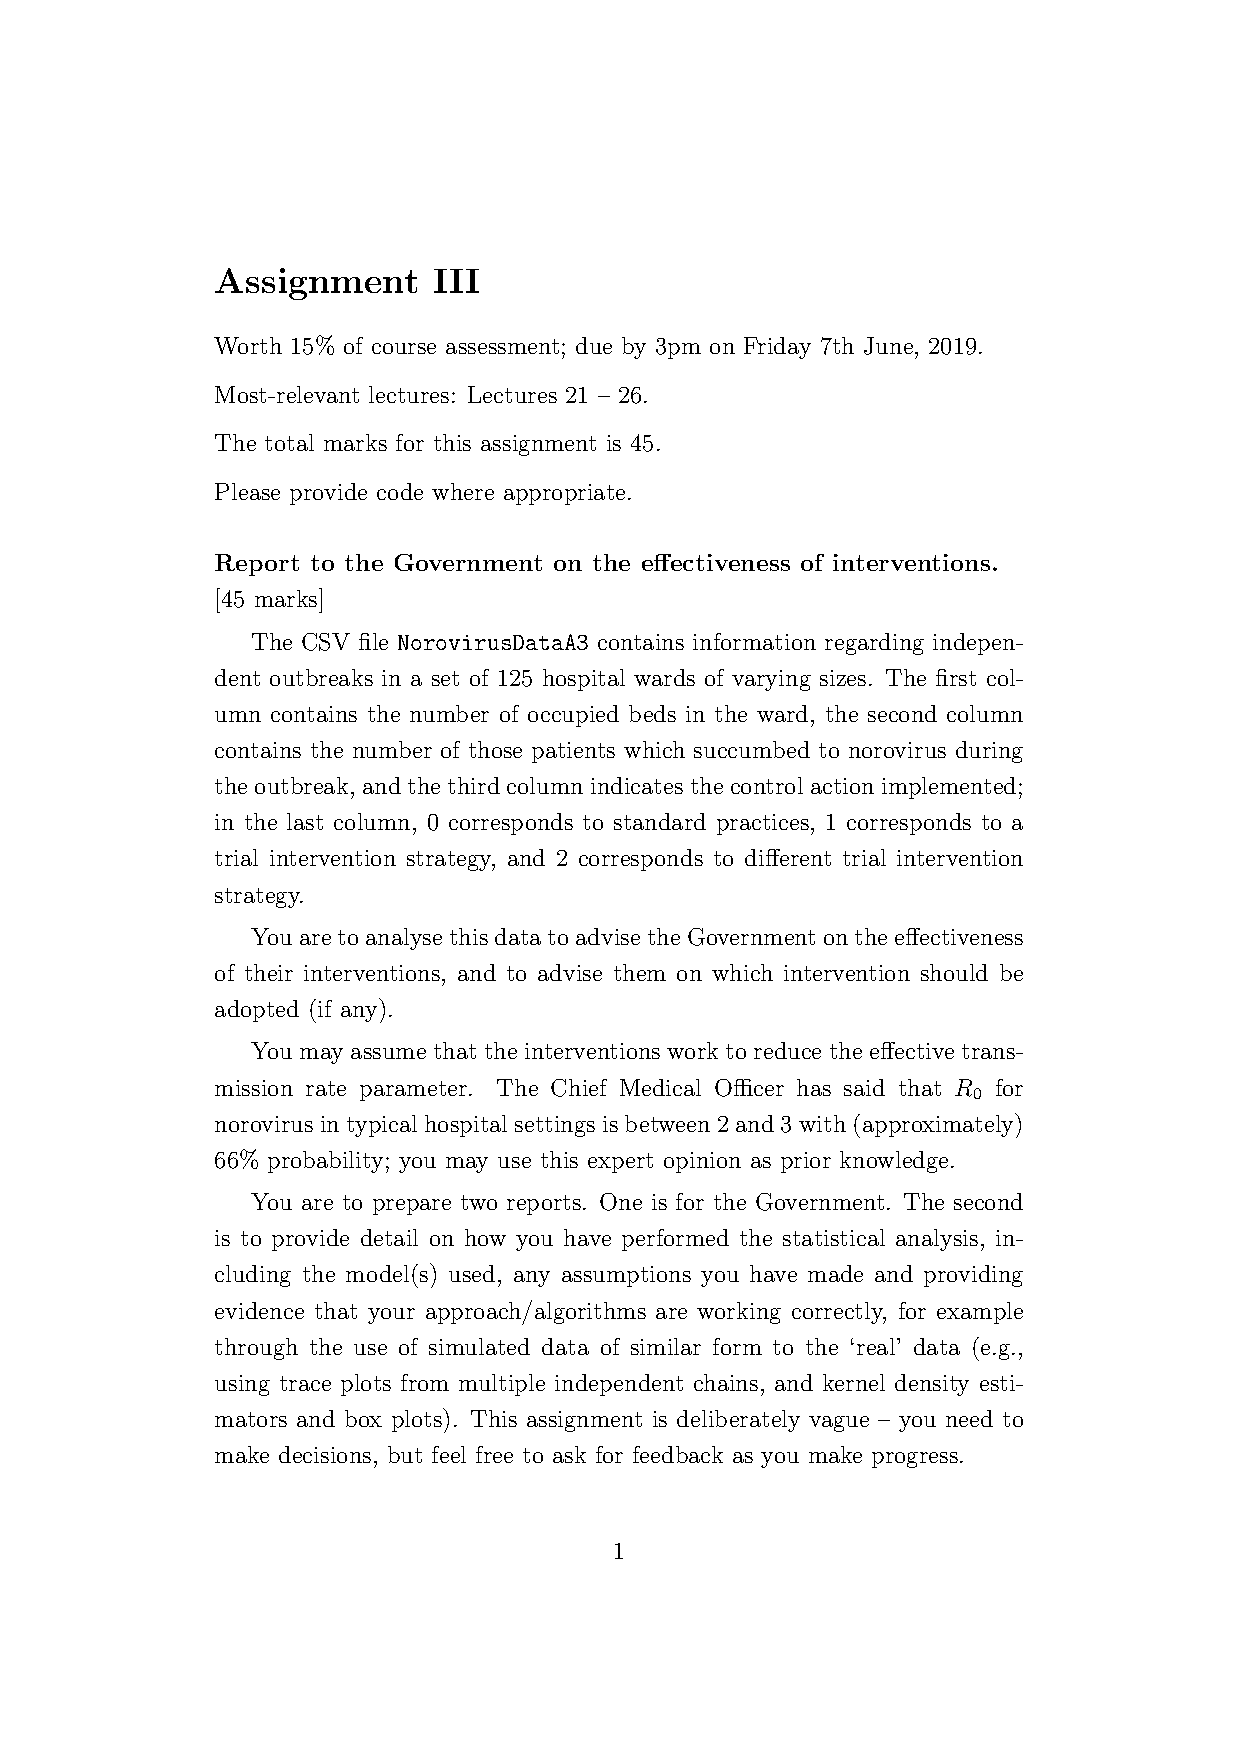
\includepdf[pages=1-]{Honours2019Assignment3}
\end{document}